\documentclass[10pt,usletter]{article}
\usepackage[letterpaper, hmargin=0.75in, vmargin=0.75in]{geometry}
\usepackage{graphicx}
\usepackage[hyphens]{url}
\usepackage{hyperref}
\usepackage{listings}
\usepackage{pgf}
\usepackage{courier}
\usepackage{amsfonts,amssymb,amsmath,amsthm,lastpage,fancyhdr,wrapfig,multirow}
\usepackage{palatino}
\usepackage{amsmath}
\usepackage{parallel,enumitem}
\usepackage{cancel}
\usepackage[english]{babel}
\usepackage{soul}
\usepackage[utf8]{inputenc}
\usepackage{fancyhdr}
\textwidth 7.5in
\oddsidemargin -.5in
\topmargin -0.70in
\textheight 9.8in                      

\pagestyle{fancy}

%**************Fill in your ID and initials here*****************
\newcommand{\mc}[1]{\ensuremath{\mathcal{{#1}}}}
\newcommand{\mb}[1]{\ensuremath{\mathbb{{#1}}}}
\newcommand{\mf}[1]{\ensuremath{\mathfrak{{#1}}}}
\newcommand{\N}[1]{\ensuremath{\{1,\ldots,{#1}\}}}

\newcommand{\Worth}[1]{\{{#1} marks\}}
\newcommand{\Sln}{\smallskip \textbf{Solution.} }
\newcommand{\Extra}[1]{\{Extra credit: {#1} marks\}}


\setlength{\parskip}{0.15in}
\setlength{\parindent}{0in}


\newcommand{\NP}{\newpage \vspace*{-0.4in}}
\newcommand{\FP}{\vspace*{-0.6in}}
\newcommand{\tab}[1][1cm]{\hspace*{#1}}

\lstset{ %
language=Java,
basicstyle=\ttfamily\scriptsize,commentstyle=\scriptsize\itshape,showstringspaces=false,breaklines=true}


\title{\huge SE465 Notes}
\author{Minyang Jiang}
\date{\today}

\begin{document}
\maketitle
\NP
\subsection{Example 1}
\begin{lstlisting}[language=Java]
static public int findLast(int[] x, int y) {
	for (int i = x.length - 1; i > 0; i--) {
		if (x[i] == y) {
			return i;
		}
	}
	return -1'
}
@Test
public void testFindlast() {
	int[] x = new int[] {2, 3, 5};
	assertEquals(0, FindLast.findLast(x, 2));
}
\end{lstlisting}
\begin{enumerate}
\item Identify and fix the fault \\
\tab for loop condition should be $i \geq 0$
\item If possible, identify a test case that does not exercise the fault \\
\tab x is null
\item if possible, identify a test case that exercise the fault, but no error state \\
\tab findLast([1, 2, 3], 2) will return -1
\item if possible, identify a test case that results in an error, but no failure \\
\tab trying to findsomething not there ([2], 5)
\item Identify the first error state
\end{enumerate}

\subsection{Example 2}
\begin{lstlisting}[language=Python]
class LineSegment:
	def __init__(self, x1, x2):
		self.x1 = x1; self.x2 = x2;
		
	def intersect(a, b):
		return (a.x1 < b.x2) & (a.x2 > b.x1);
\end{lstlisting}
Establishing correctness of intersect:
\begin{enumerate}
\item[•] case analysis of the inputs
\end{enumerate}
Other answers
\begin{enumerate}
\item[•] execute every statement of the unit under test
\item[•] feed random inputs
\item[•] check all outputs
\item[•] check values of each clause
\end{enumerate}
rename inputs: \\
$a = a.x_1 \tab b = b.x_1$\\
$A = a.x_2 \tab B = b.x_2$
\begin{enumerate}
\item[-]assume all points are distinct\\
\item[-]assume $a < b$ (we'll check both ways when constructing test cases) \\
\item[-]assume $a < A, b < B$
\end{enumerate}
aAbB\\
abAB\\
abBA
\begin{lstlisting}[language=Python]
# run this test as 'python line-intersection-test.py'

from line_intersection import *
import unittest

class TestIntersection(unittest.TestCase):
    def test_aAbB(self):
        a = LineSegment(0,2)
        b = LineSegment(3,7)
        self.assertFalse(intersect(a,b))
        self.assertFalse(intersect(b,a))

    def test_abAB(self):
        a = LineSegment(0,4)
        b = LineSegment(3,7)
        self.assertTrue(intersect(a,b))
        self.assertTrue(intersect(b,a))

    def test_abBA(self):
        a = LineSegment(0,4)
        b = LineSegment(1,2)
        self.assertTrue(intersect(a,b))
        self.assertTrue(intersect(b,a))

    def test_equality(self):
        a = LineSegment(0,2)
        b = LineSegment(2,4)
        self.assertTrue(intersect(a,b))        # A = b
        self.assertTrue(intersect(b,a))        # B = a
        a = LineSegment(2,2)
        b = LineSegment(0,4)
        self.assertTrue(intersect(a,b))        # a = A
        self.assertTrue(intersect(b,a))        # b = B
        a = LineSegment(0,2)
        b = LineSegment(0,4)
        self.assertTrue(intersect(a,b))        # a = b
        self.assertTrue(intersect(b,a))        # b = a

if __name__ == '__main__':
    unittest.main()

\end{lstlisting}

\subsection{•}
\noindent
\fbox{
\begin{minipage}[t]{0.48\linewidth}
Static:
\begin{enumerate}
\item[-] find faults\\
example:
\begin{enumerate}
\item type checking
\item dead code analysis
\end{enumerate}
\item[-] code inspection functionality and style
\item[-] program verification
\end{enumerate}
\end{minipage}}
\hfill%
\fbox{
\begin{minipage}[t]{0.48\linewidth}
Dynamic
\begin{enumerate}
\item[-] observe failures
\item[-] must generate inputs\\
\tab what are expected outputs?
\item[-] easy to run the program
\item[-] keywords\\
\tab white-box testing\\
\tab black-box testing
\end{enumerate}
\end{minipage}}

static techninques tradeoff:
\begin{enumerate}
\item[-] exhaustive 
\item[-] subject to false positives
\end{enumerate}

words I don't like \\
\tab \st{complete testing}\\
\tab \st{exhaustive testing}\\
\tab \st{full coverage}

First big question: When should I stop testing?
\begin{enumerate}
\item when I run out of time\\
\tab open-ended explorotroy testing\\
\tab for automatic input generation
\item when I'm close enough to being exhaustive\\
\tab explored enough (all) of \\
\tab[2cm] behaviours / use cases\\
\tab[2cm] program states\\
\tab[2cm] inputs\\
\tab[2cm] statements / branches
\end{enumerate}

\huge{observability, controlability}
\subsection{Coverage}
\normalsize
\begin{enumerate}
\item[-] idea: find reduced space + cover it with test cases
\end{enumerate}
Test Requirement (TR) - an element of an artifact that soe test case must satisfy

\section*{Infeasible Test Requirements}
unreachable code
definition: coverage level - Given a set of test requirements TR and a test set T, The \underline{coverage level} is the ratio of the number of TRs satisfied by T to the size of TR.

\subsection*{Exploratory Testing}
\begin{enumerate}
\item[-] usually carried out by testers
\item[-] unscripted in general\\
\tab "Exploratory teesting is simulatneous learning, test design, and test execution"
\end{enumerate}
\subsection*{Exploratory testing is good for}
\begin{enumerate}
\item[-] simulating actual use cases (realism)
\begin{enumerate}
\item[-] diversifying testing beyond scripts
\end{enumerate}
\item[-] finding single most important bug in sortest time
\item[-] being less siloed
\item[-] evaluating aparticular risk, see if scripted tests needed
\end{enumerate}
\subsection*{Exploratory Testing Process}
\begin{enumerate}
\item start with a goal /charter
\begin{enumerate}
\item[•]"Explore the product elements"
\end{enumerate}
\item decide which area of the software to test
\item design a test (informally)
\item execute test and log bugs
\item repeat as needed
\end{enumerate}
notes: don't produce exhaustive notes
output: \begin{enumerate}
\item set of bug reports
\item test notes (possibly a judgment)
\item artifacts (input, output)
\end{enumerate}
\subsection*{\underline{Results of WaterlooWorks Testing}}
\begin{enumerate}
\item sort order reversed on navigating to subsequent page
\item use of ophrase "current term" is ambiguous when choosing a term
\item on mobile, sort order not preserved when navigating to a job posting and going back
\end{enumerate}
\underline{Overall}
\begin{enumerate}
\item want some sort of judgment on overall usability of system\\
\tab do the primary functions work well enough
\end{enumerate}
\subsection*{Control flow graphs}
Coverage criteria for source code\\
stream of characters $\rightarrow$ stream of tokens $\rightarrow$ abstract syntax tree $\rightarrow$ control flow graph\\
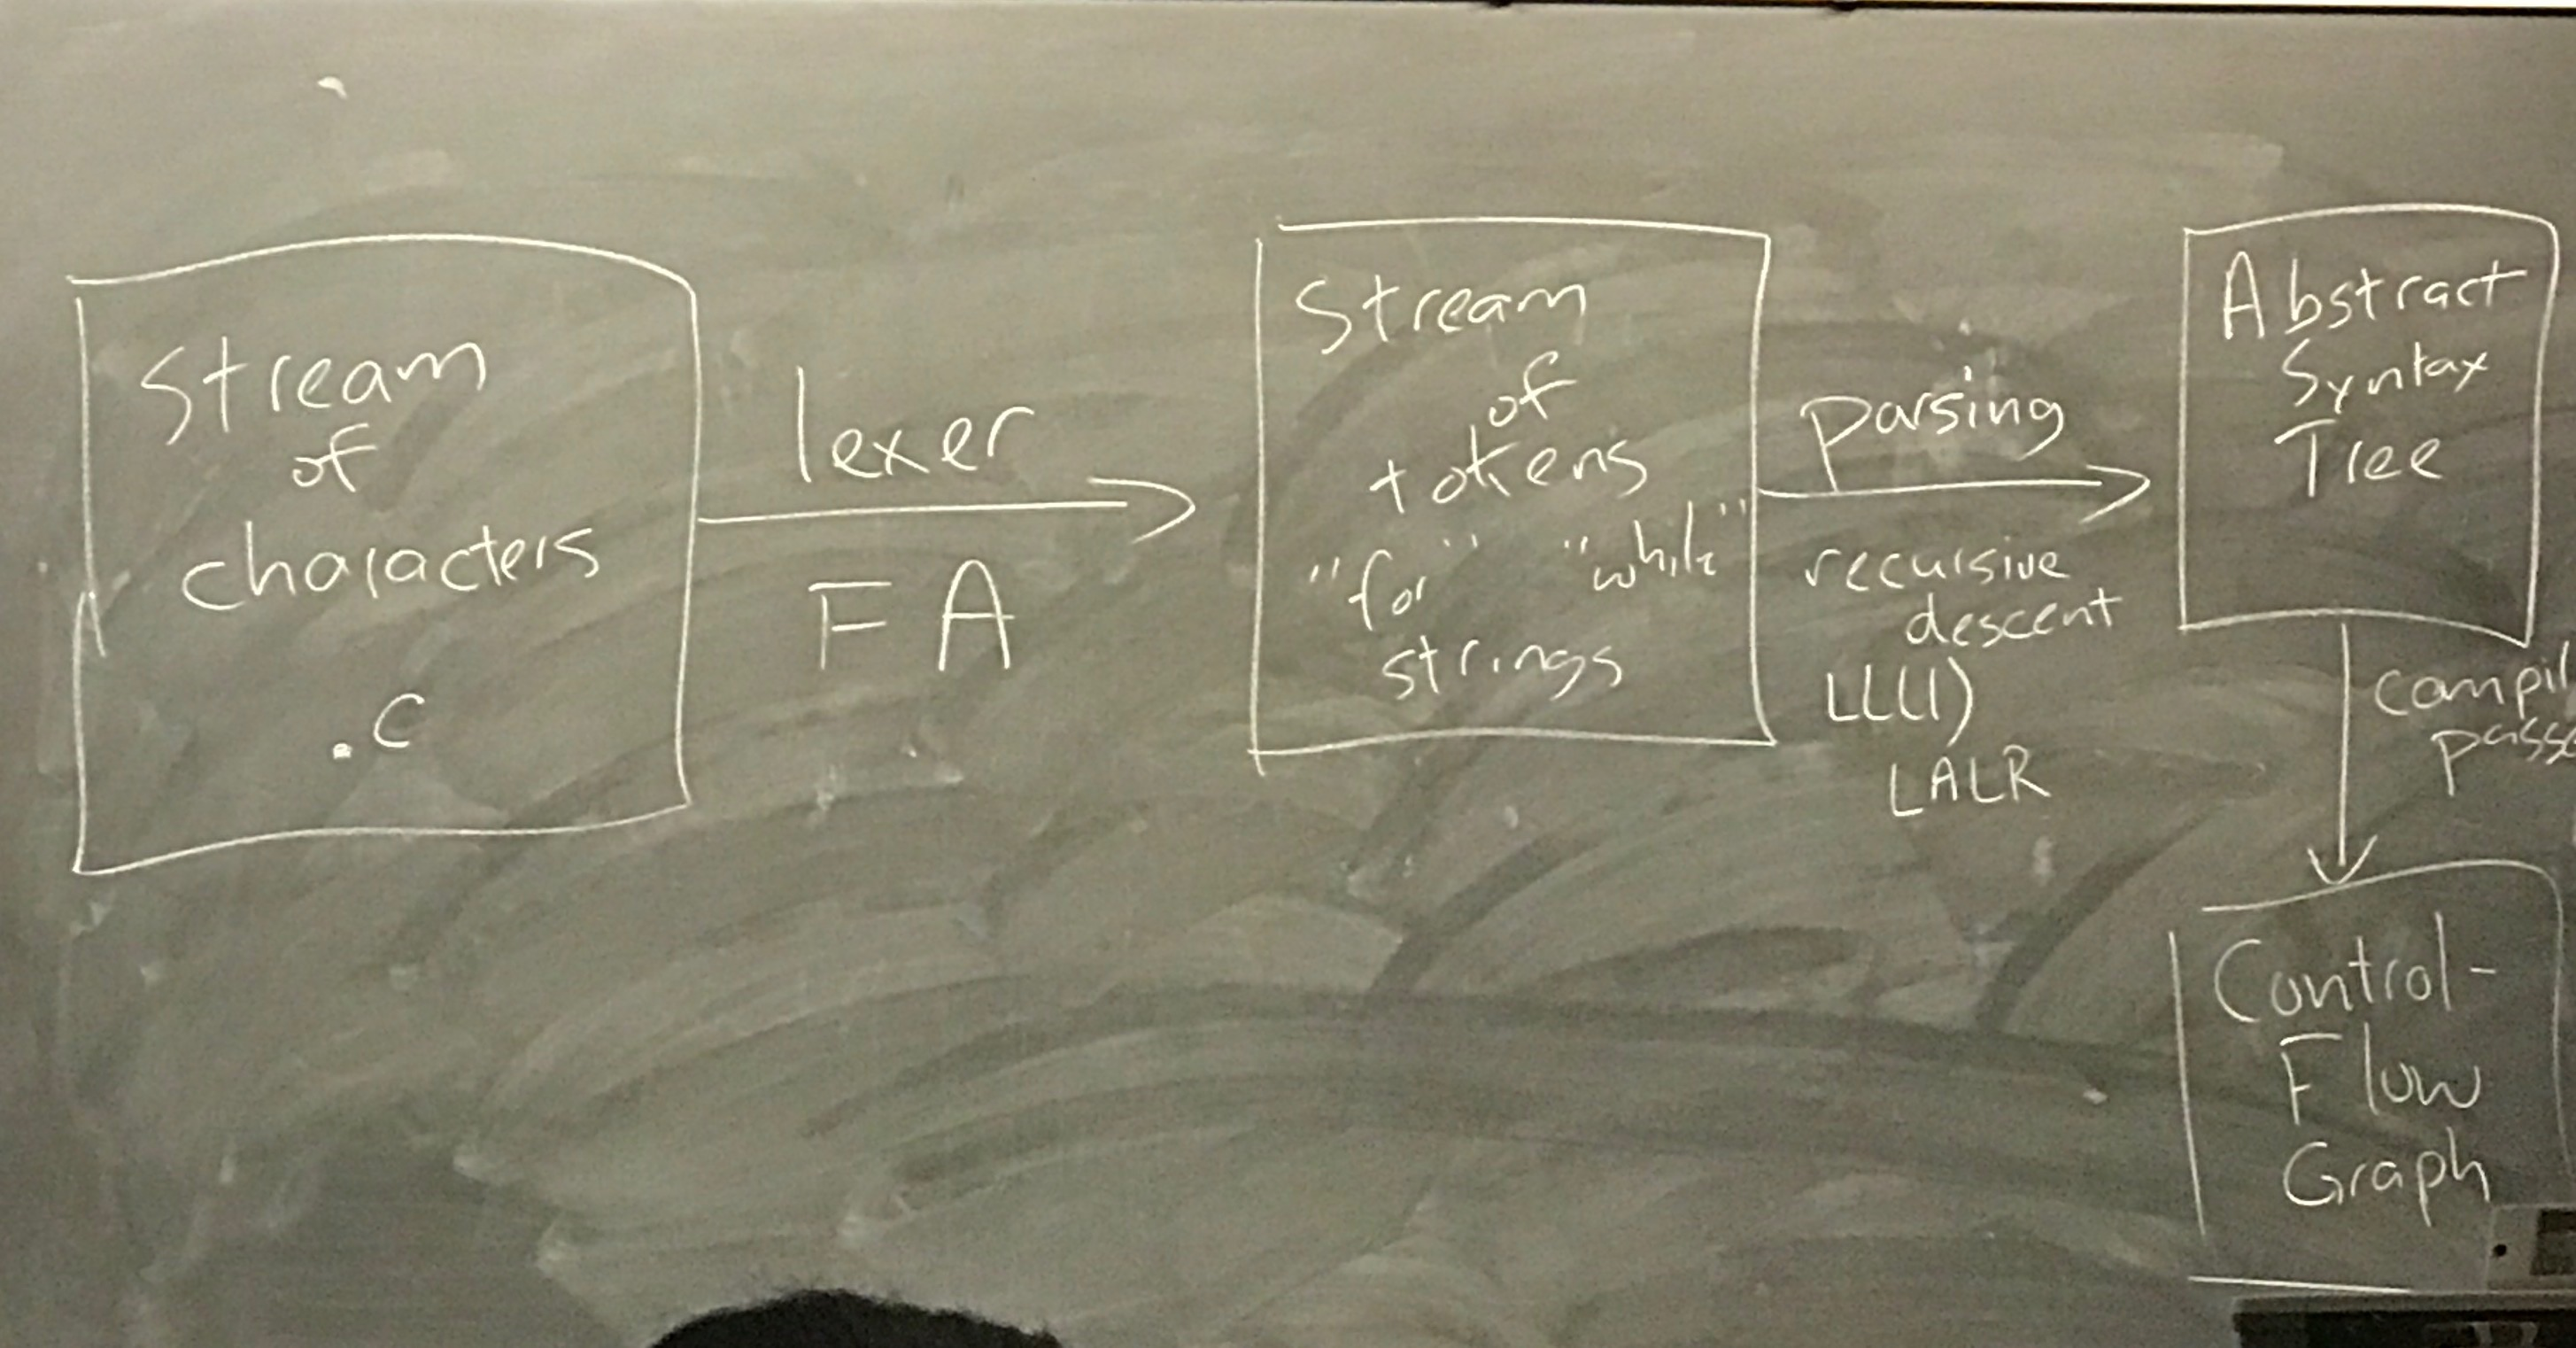
\includegraphics[scale=0.1]{control_flow_graph_1}\\
\underline{Control Flow Graph}
\begin{enumerate}
\item representation of program which is easier to analyze\\
\tab Nodes: represent 0 or more statements\\
\tab Edge (directed) $(s_1, s_2)$ means $s_2$ may follow $s_1$ in an execution
\end{enumerate}


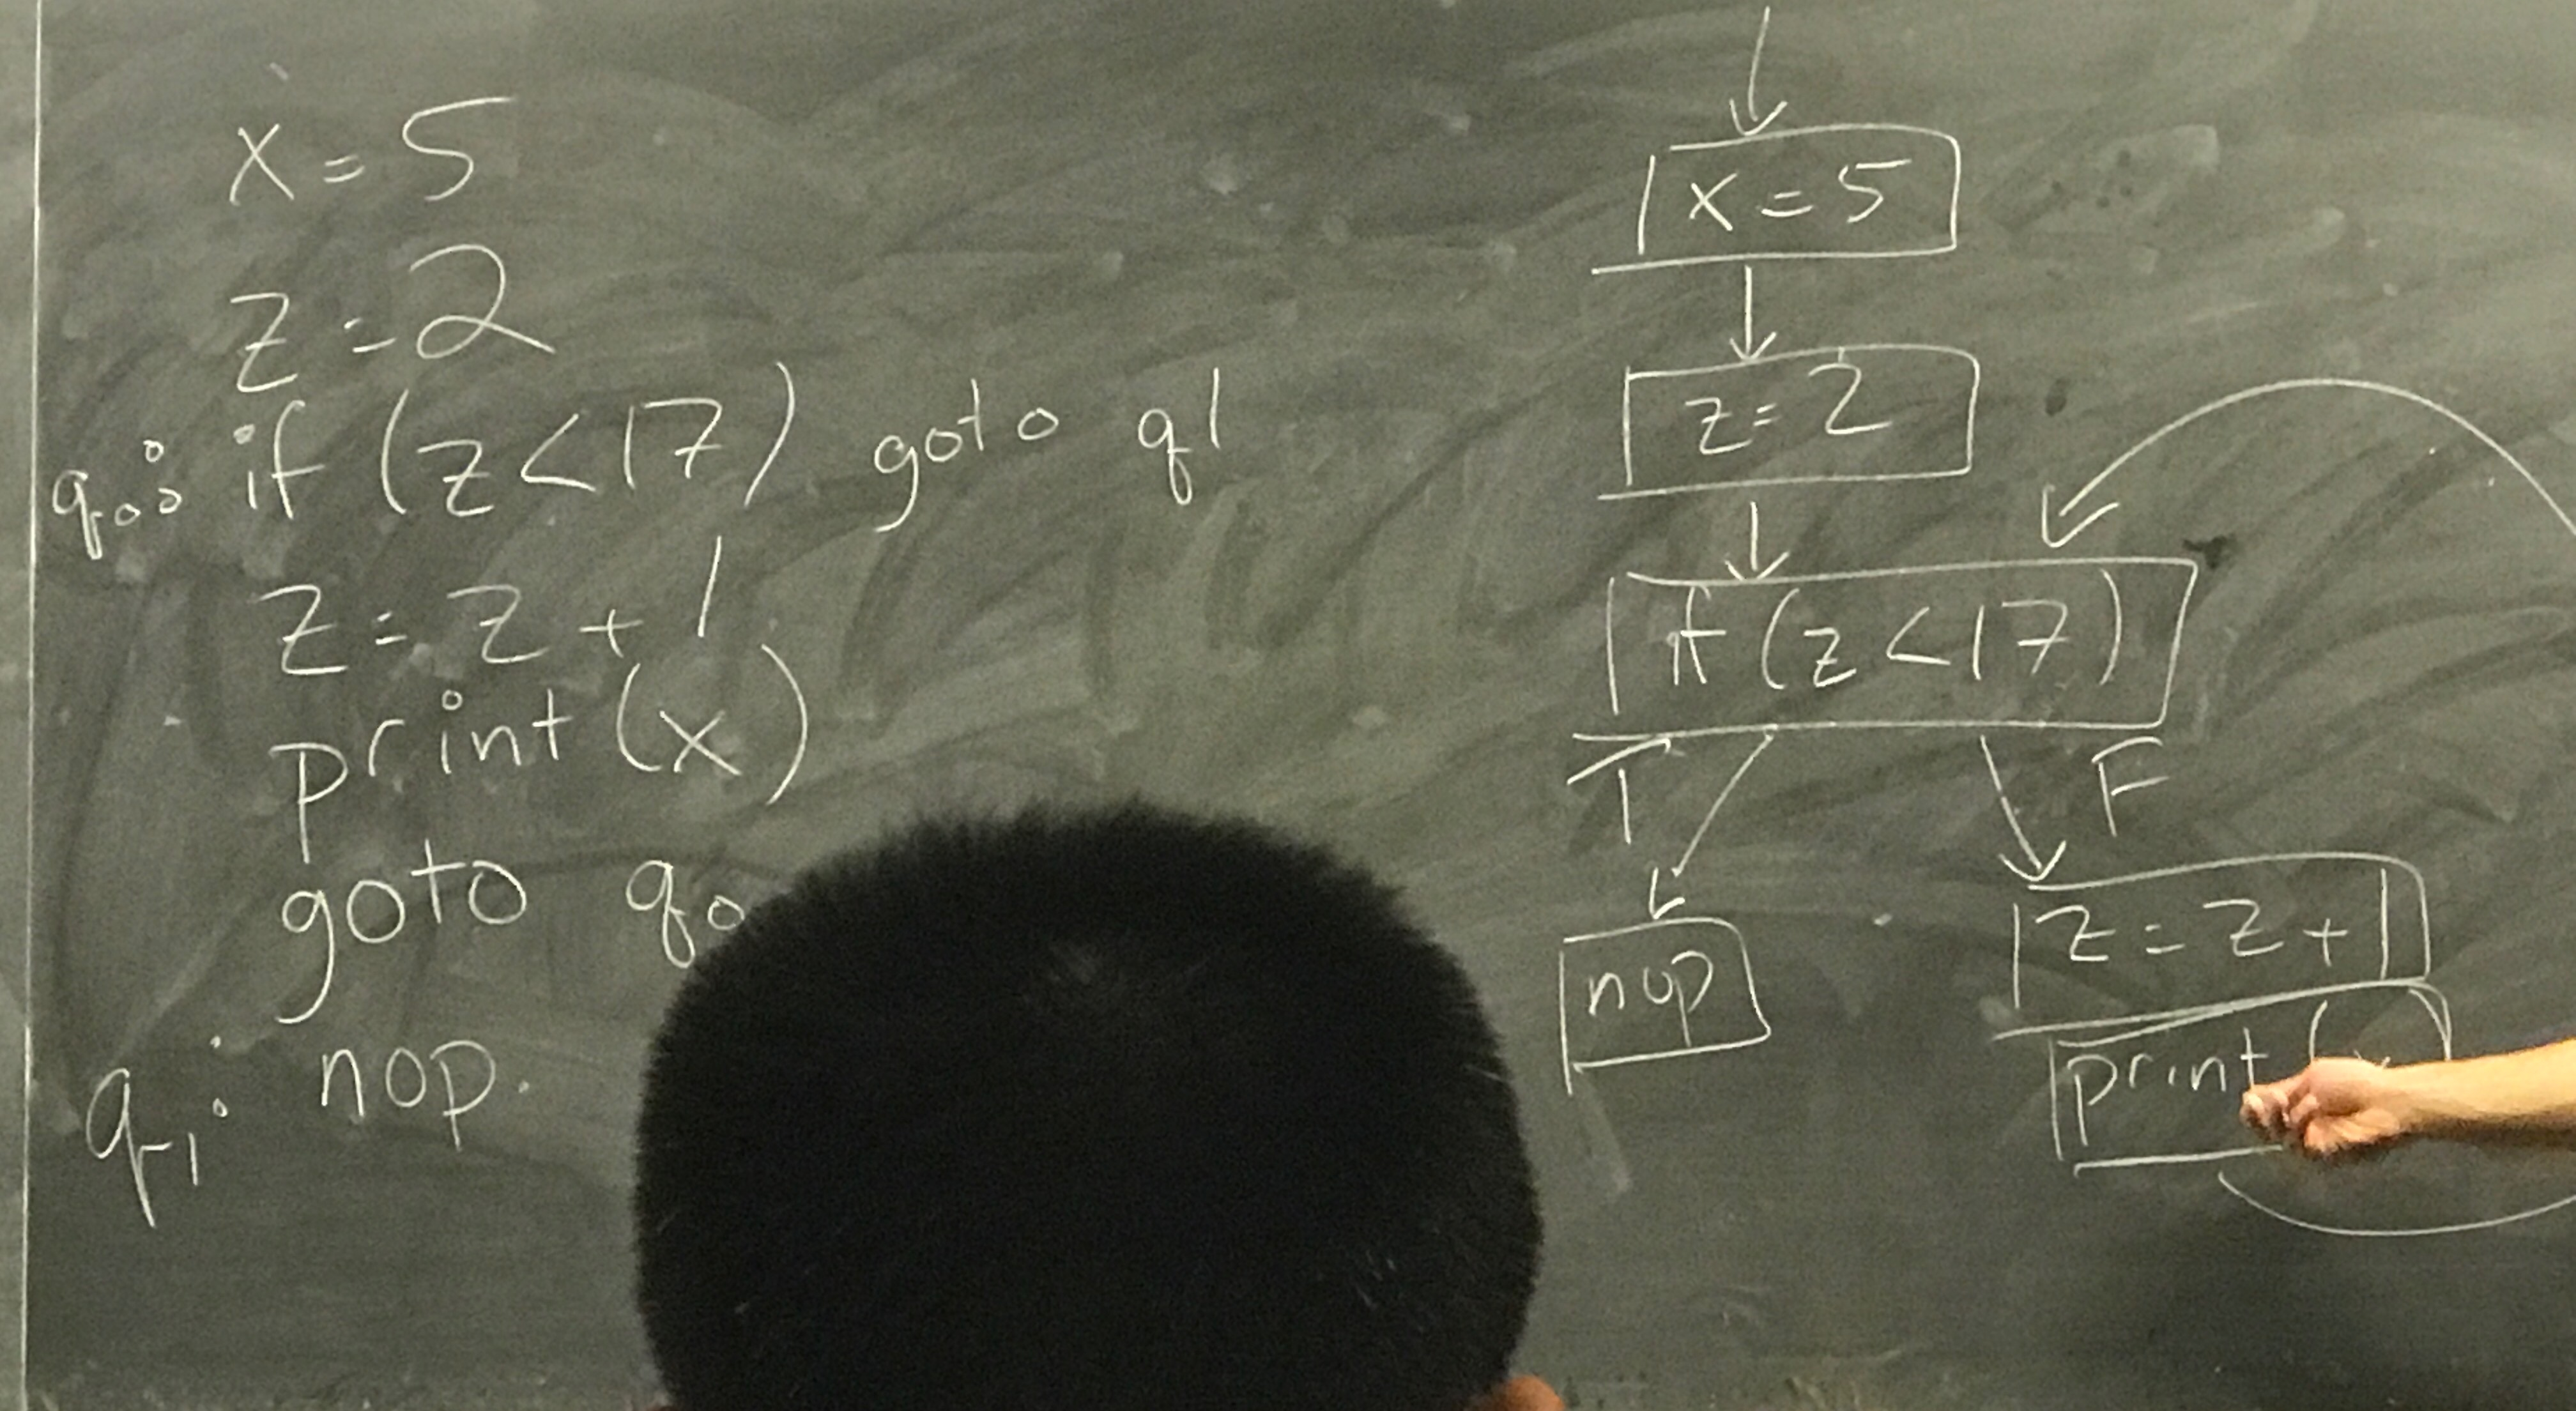
\includegraphics[scale=0.1]{control_flow_graph_2}\\

Basic Blocks: A \underline{basic block} has one entry point and one exit point and is maximal \\


\subsection{Statement and Branch coverage}
Definition: A \underline{test path} is a path p that starts at an initial node and ends at final node\\
Given a set of test requirements TR, for a graph criterian C, a test set T satisfies C on graph G iff for every test requirement tr in TR, at least one test path P in path (T) exists such that P satisfies tr\\
\underline{Test paths + test cases}
\begin{enumerate}
\item when testing , you provide test cases asa inputs to the program
\item each test case t gives at least one test path, path(t)
\item test set T = set of test cases path(t) = \{path(t) $\vert$ t $\in$ T\}
\end{enumerate}
Test Requirement:\\
\tab a condition that a test path may satisfy\\
Coverage criteria:\\
\tab generate sets of test requirements given graphs or other artifacts\\
Statement Coverage:\\
\tab have one test requirement for each node in the CFG\\
cause of nondetermminism:\\
\tab dependence on inputs, on thread scheduler, on memory addresses\\
Results: one input may give multiple outputs and multiple test cases

\underline{Review: Coverage Criteria}\\
criterian + graph \\
statement coverage $\Rightarrow$ set of test requirements\\

Test set = Bunch of inputs to SUT(system under test)\\
test cases t $\in$ T,\\
execution givs path (T), check how many test requirements path (T) satisfied\\

Criterion- Compute Path Coverage\\
TR contains all paths in G\\
Is infeasible when you have loops in G\\

\underline{Next: Finite- State Machines}\\
CFG: generate directly from source code\\
FSM: higher level, usually represent some design information\\
Example:\\
\tab navigation structure of webapp\\
Nodes: software states (variable values, or pages)\\
edges: transitions between software states (e.g. as triggered by the user with commands, or triggered by the passage of time)\\

\underline{Criterian Simple Round Trip Coverage (SRTC)}\\
TR contains at least one round-trip path for each reachable node in G that begins and ends a round-trip path\\
complete round-trip coverage: Like STRC, but "at least one" $\Rightarrow$ "all"\\
Defn A \underline{round-trip path} is a path of nonzero length with no internal cycles that starts and ends at the same node.\\

\underline{Deriving FSMs}\\
\begin{enumerate}
\item no good mechanical ways to get good FSMs
\item must understand the system\\
\tab will see some tools that help - comments 
\end{enumerate}
CFGs - poor way of getting FSMs\\
large + unwieldy\\

Sources of FSMs:
\begin{enumerate}
\item CFGs terrible
\item better: design docs / software structure	
\end{enumerate}
FSMs from software structure
\begin{enumerate}
\item requires lots of efforts
\item subjective
\item need to know the 
\end{enumerate}
FSMs from storeed state
\begin{enumerate}
\item identify key variables summarizing system state
\item values of variables determine state
\item changes in variables result in changes in state can be more mechanical than FSM from structure
\end{enumerate}

\underline{Generally:}\\
FSMs enable
\begin{enumerate}
\item test descriptions to be created before implementation FSMs easier to analyze than code
\end{enumerate}
But:
\begin{enumerate}
\item not exhaustive
\item doesn't necessarily match the implementation
\end{enumerate}

\underline{Syntax-based Testing}\\
\begin{enumerate}
\item input space grammars
\item mutation-based testing
\end{enumerate}

credit card numbers \\
Hover, there is a check sum, and many \#s conform to the regex but are semantically invalid\\
Idea: use the regexp to generate syntactically valid \#s then need to filter based on checksum to set valid \#s\\
Question: how to generate syntactically invalid id \#s?
\begin{enumerate}
\item modify the regexp to generate invalid \#s , e.g. super long \#s
\item change somthing while generating the string
\end{enumerate}

Instead of regex, can use context free grammars using grammears:
\begin{enumerate}
\item generate vallid and invalid program inputs
\item inside program validate input
\end{enumerate}

Generators:\\
Start with start production\\
replace non terminals with what's on RHS eventually set strings belonging\\
repeat until you have enough input language
\\
\underline{A grammar}
roll = action\\
action = dep|deb\\
dep = \"deposit\" account amount\\
dep = \"debit\" account amount\\
account = digit 33\\
amount = \$ digit + . digit\\
digit =[0-9]\\
\underline{Grammar mutation operators:}\\
Specific example - make acount a 4 digit number\\
more generally: 
\begin{enumerate}
\item add new non termminals to existing productions
\item remove existing nonterminals from productions
\item permuting nonterminal order within a production
\end{enumerate}
Everything we said with nonterminals also applies for terminals e.g. \$, .\\

\underline{Fuzzing}\\
Fuzzing actually works\\
\tab -specifically for security bugs\\

\underline{Origin Story}
\begin{enumerate}
\item Line noise for 1200 band moderms
\item fragile 1988 unix utils would crash on bad inputs
\item Prof Barton Miller challanged his os class to generate random ASCII inputs
\item they crashed 25-30 of unix utils
\end{enumerate}

\underline{more on fuzzing}\\
\tab Two kinds: mutation-based\\
\tab\tab generation-based\\

mutation-based fuzzing:\\
\tab modify existing test cases to generate new behaviours\\
generation-based testing\\
\tab start with a grammar, generate inputs that match grammar\\
what to do with generating inputs: (ie what is correct output?)
\begin{enumerate}
\item can look for crashes/assertion failures\\
\item can run under dynamic analysis tools (Valgrind)
\end{enumerate}
In practice: the simplest thing that could work:\\
HTML5: regexp (.*) random bit, finds webkit assertion failure\\
process generate random strings put them in a file ask browser to open them\\

More sophisticated fuzzing:\\
\tab C programs:
\begin{enumerate}
\item sequence of ASCCII chars
\item sequence of words, separators and white space
\item syntactically correct C program
\item type-correct C program
\item statically - fonforming C programs, e.g. must have main 
\item dynamically conforming C programs, e.g. no invalid memory access
\item model conforming C programs (even stranger than 6, exact details unimportant)
\end{enumerate} 
As we descent, we are more likely to find bugs specific to the system (e.g. C compiler)\\
Mutation-based Fuzzing
\begin{enumerate}
\item modify existing inputs
\begin{enumerate}
\item randomly flip bytes
\item or parse the input and thenn change some nonterminals
\end{enumerate}
\item usually need to update applicable check sums
\end{enumerate}
Fuzzing Summary:
\begin{enumerate}
\item useful technique for finding interesting tets cases
\item advantageL runs automatically and really works!
\item disadvantages: need work to find deeper case
\end{enumerate}
Related: Chaos Monkey
\begin{enumerate}
\item distributed system
\begin{enumerate}
\item parts fail
\end{enumerate}
\end{enumerate}
Industry:\\
\tab 80\% statement coverage\\
\tab no quantitative measurement of input space\\
\tab $\rightarrow$ stop when you don't find new bugs\\
now: JUnit case study
\begin{enumerate}
\item why not 100\%
\item should be a best practice
\end{enumerate}
overall stats:
\begin{enumerate}
\item 85\% statement coverage
\item 13,000 lines of code system
\item 15,000 lines of code test
\end{enumerate}
\underline{Deprecated code}:\\
-might go away soon \\
JUnit: 65\% coverage in deprecated classes, 93\% otherwise\\
One JUnit class was completely untested
\begin{enumerate}
\item tests were included originally, but never actually executed
\end{enumerate}
What else -- the usual suspects
\begin{enumerate}
\item too simple to test\\
\end{enumerate}
\underline{Dead by design}
\begin{enumerate}
\item constructors on classes not to be instantiated (e.g. containers of static methods)
\item code that should never be executed
\item code that is too difficult to trigger
\end{enumerate}
conclusions:
\begin{enumerate}
\item remember coverage does not guarantee rests are good
\item non-deprecated code, 93\% coverage, no more than 2-3 lines untested code
\end{enumerate}
\subsection*{Mutation Testing}
the question: is your test suite any good?\\
How to tell?\\ 
\tab Try modifying your program and see if the test suite notices\\
grammar = programming language grammar
Def: \\
\tab Ground String - a valid string belonging to the language of the grammar (original program in other words)\\
\tab Mutation operator- rule that specifics syntactic variations of strings generated from a grammar\\
\tab Mutant- result of applying mutation operator to ground string\\

mutation is hard to apply by hand (systematically) and har to automate - can't tell whether you actually changed the program\\
mutation = gold standard benchmark - compare other criteria to it\\
Killing Mutants: \\
1.original program = $m_0$\\
2.apply mutation operator, get mutant $m_i$\\
Definition:\\
\tab test case t kills m if running t on m gives different output than running t on $m_0$\\
Mutation score = \% of mutants killed\\
using mutation testing: fix a se of mutants and keep adding tests until score reaches target.\\
\underline{Mutation Testing and Programs}
use mutation ops to modify program\\
mutant = valid \underline{program} which behaves differently from original program\\
task when mutation testing = create tests which distingguish mutants from originals\\

\begin{enumerate}
\item create a mutant
\item find a test case that kills the mutant
\item forget the mutant keep the test case
\end{enumerate}

\underline{uninteresting mutants}
\begin{enumerate}
\item still born - cannot compile or immediately crash
\item trivial - killed by almost any test case
\item equivalent - always behaves some as original
\end{enumerate}
Goals of mutation Testing
\begin{enumerate}
\item mimic typical mistakes
\item force inclusion of some kinds of tests\\
\tab stmt coverage via bomb\\
\tab checking for 0 (insert fail on zeros)
\end{enumerate}
\underline{Weak us strong mutation}
so far, kill a mutation by producing\\
\tab we will call this "strong mutations" output\\
notion of "weak mutation"\\
\tab error state need not be output
\\
How to test weak mutation?
print out internal state (compare it)\\
need about same \#tests for weak strong mutation

"73\%"
\begin{enumerate}
\item out of the set of 300+ real bugs
\item the mutator they generated found 73\% of these bugs
\end{enumerate}

Why tests?
\begin{enumerate}
\item anecdote - write a Java server to interface with Android app
\begin{enumerate}
\item set up dev server at dev machine
\item install app on a test phone
\item manually create case on test phone
\item was forced to write test cases to pass code review
\item later, had to do a bug fix\\
\tab test cases ensured that nothing else got broken
\end{enumerate}
\end{enumerate}


































\end{document}